\documentclass[12pt,a4paper]{article}

\usepackage[utf8]{inputenc}
\usepackage[english]{babel}
\usepackage{a4wide}
\usepackage{index}
\usepackage{blindtext}
\usepackage[graf, intHoriz, sinLU, showDirectores]{../assets/caratula}

\usepackage{amsmath}
\usepackage{amssymb}
\usepackage{bm}
\usepackage{hyperref}
\usepackage{tikz}
\usepackage[dvipsnames]{xcolor} % more colors

\usepackage{adjustbox}
\usepackage{multirow}
\usepackage{array}
\usepackage{makecell}
\usepackage{subfig}

% chess typesetting
\usepackage{skak}
\usepackage{xskak}
\usepackage{wasysym} % other symbols

\usepackage{csquotes}
\usepackage[backend=biber]{biblatex}
\addbibresource{../refs.bib}

\integrante{Martín Emiliano Lombardo}{}{mlombardo9@gmail.com}
\titulo{Análisis de feature sets con redes neuronales NNUE para engines de ajedrez}
\fecha{\today}
\materia{}
\director{Agustín Sansone}{agustinsansone7@gmail.com}
\director{Diego Fernández Slezak}{dfslezak@dc.uba.ar}

\makeindex

\begin{document}

\maketitle

\tableofcontents
\newpage

\section{Introduction}

% The rise of NNUEs
% https://stanford.edu/~cpiech/cs221/apps/deepBlue.html

% https://deepmind.google/discover/blog/alphazero-shedding-new-light-on-chess-shogi-and-go/
% https://crimsonpublishers.com/cojra/pdf/COJRA.000563.pdf
% https://arxiv.org/pdf/2209.11902.pdf

The development of chess engines was and continues to be a topic of study in the chess and computer communities for decades. IBM DeepBlue \cite{deepblue:2002} was the first chess machine to reach superhuman level by consistently beating the world champion, Garry Kasparov, in 1997 \cite{washingtonpost:1997}. Since then, engines have evolved in strength and complexity. \\

Chess can be modeled as a tree, where each node is a particular board configuration and the edges are legal moves for that position. With this representation, engines can use tree search algorithms to explore the tree and approximate the best move. Since the 1950s and to this date, engines have used algorithms like Minimax \cite{minimax-survey:1995} and Monte Carlo Tree Search \cite{mcts-survey:2012} (MCTS) or some of its variants \cite{tree-search-methods:2014,mcts-modifications:2022} to accomplish this.

The number of possible positions in chess is vast, estimated by Shannon \cite{shannon:1950} to be around $10^{43}$. This number is based on the average number of legal moves per position and the average game length. This makes it not feasible to explore the entire tree, so every tree search algorithm relies on having an evaluation function: a function that takes the state of the game and returns a single real number. This number is used to encompass information about the whole subtree of that position so it can be propagated up the tree, depending on the algorithm. Until a few years ago, highly complex handcrafted functions were used that were based on human knowledge about the game. \\

Until the 2010s, the development of engines advanced at a slow but consistent pace. Until 2017 that Google DeepMind published AlphaGo Zero \cite{alphagozero:2017} and its successor AlphaZero \cite{alphazero:2017,alphazero:2018} in 2018, which proved to be overwhelmingly superior (28 wins, 73 draws and 0 losses against the best engine at that time). They introduced a new approach to the development of board game engines, including chess: train a convolutional neural network with a reinforcement learning algorithm to learn to play by itself.

This change of paradigm, where the evaluation of positions is done by neural networks instead of functions built with human knowledge, altered the course of development of all modern engines (not just Go and chess). In 2018, Yu Nasu introduced the networks \reflectbox{EUNN} (or NNUE) ``Efficiently Updatable Neural-Networks'' \cite{nnue:2018} for the game Shogi. NNUE networks allow for cheap evaluations when evaluating a sequence of similar positions, making them ideal for use in depth-first search based engines. Since then, all modern engines have incorporated NNUE networks or some kind of neural network in their evaluation.

The chess engine Stockfish \cite{stockfish}, modern successor of DeepBlue with improved heuristics and running in commercial hardware is one of the strongest in the world. It incorporated NNUE networks mixed with classical evaluation in version 12\footnote[1]{\href{https://stockfishchess.org/blog/2020/introducing-nnue-evaluation/}{Introducing NNUE evaluation (Stockfish 12)}}. Since Stockfish 16.1\footnote[2]{\href{https://stockfishchess.org/blog/2024/stockfish-16-1/}{Removal of handcrafted evaluation (Stockfish 16.1)}} (2024) the evaluation is done exclusively through NNUE networks, eliminating all human aspect.

\newpage
\subsection{Thesis plan}

The main goal of this thesis is to explore different kinds of board encodings called feature sets. These encodings are the input for a NNUE network. To do so, I need a chess engine that supports neural networks with the ability to customize encodings and a way to train them.

I decided to implement a simple but capable classic engine based on well-known algorithms and optimizations, and then change the evaluation to use NNUE networks, with a versatile framework to build feature sets. Finally, I implemented a training pipeline to train the networks and measure their performance.

With the setup ready, I run multiple experiments. I propose different feature sets, train networks with them and compare their performance.

% The initial idea was to use Stockfish with the official Pytorch trainer \cite{nnue-pytorch}. However, I quickly realized that implementing some of the features sets I had in mind may be too complicated  with Stockfish's representation and the unconventional training test (PQR) that I wanted to do was impossible. This, and given that Stockfish engine and trainer codebases are huge, I felt there was too much magic involved so I turned away. I could have picked up another less complex engine written in Rust (like Marlin) and modify it, but I choose not to.
% So, I decided to implement my own engine and training pipeline from scratch.

\subsection{Source code}

The source code for this work can be found online in the following repositories:

\begin{table}[H]
\centering
\begin{tabular}{ll}
\toprule
\textbf{Repository} & \textbf{Repository} \\
\midrule
Source code & \url{https://github.com/mlomb/cs-master-thesis} \\
\LaTeX\ documents & \url{https://github.com/mlomb/cs-master-thesis-doc}
\end{tabular}
\end{table}

\newcommand{\white}{\fullmoon}
\newcommand{\black}{\newmoon}

\newcommand{\bigtimes}{\mathop{\raisebox{-0.5ex}{\scalebox{2}{$\times$}}}}

% https://texdoc.org/serve/chessboard/0
\newcounter{pieceindex}
\newcommand{\pieceBoard}{
    \newcount\pieceindex
    \setcounter{pieceindex}{0}
    \raisebox{-7ex}{
        \centering
        \chessboard[
            tinyboard,
            showmover=false,
            margin=false,
            padding=false,
            hlabel=false,
            vlabel=false,
            pgfstyle={text},
            %text=\fontsize{1.2ex}{1.2ex}\bfseries\sffamily \thepieceindex \stepcounter{pieceindex}, %  \currentwq
            text=\fontsize{1.2ex}{1.2ex}\bfseries\sffamily \currentwq,
            markboard
        ]
    }
}
\newcommand{\pieceRolesTable}{
    \begin{tabular}{|l|}
        \hline
        \sympawn\ Pawn \\
        \hline
        \symknight\ Knight \\
        \hline
        \symbishop\ Bishop \\
        \hline
        \symrook\ Rook \\
        \hline
        \symqueen\ Queen \\
        \hline
        \symking\ King \\
        \hline
    \end{tabular}
}
\newcommand{\pieceColorsTable}{
    \begin{tabular}{|l|}
        \hline
        $\white$ White \\
        \hline
        $\black$ Black \\
        \hline
    \end{tabular}
}

\newcommand{\fs}[1]{\textsc{#1}}


\section{Feature set (board encoding)}

To evaluate chess positions, we will use a neural network with an architecture explained in detail in the next chapter. In this chapter, we will build the one-dimensional input vector for such network, which can be described entirely by a feature set.

A feature set is a set built by a cartesian product of smaller sets of features, where each set extracts a different aspect of a position. Each tuple in the feature set corresponds to an element in the input vector, which will be set to $1$ if the aspects captured by the tuple is present in the position, and $0$ otherwise. If a tuple is present in a position, we say that the tuple is \textit{active}.

Let's consider some basic sets of features. The following sets encode positional information about the board:

\begin{center}
\begin{tabular}{cc}

$\begin{aligned}[t]
\fs{File} &= \{a, b, ..., h\} \\
\fs{Rank} &= \{1, 2, ..., 8\} \\
\fs{Square} &= \{a1, a2, ..., h8\}
\end{aligned}$

&

\raisebox{-10ex}{
\chessboard[
    tinyboard,
    showmover=false,
    pgfstyle={text},
    %text=\fontsize{1.2ex}{1.2ex}\bfseries\sffamily \thepieceindex \stepcounter{pieceindex}, %  \currentwq
    text=\fontsize{1.2ex}{1.2ex}\bfseries\sffamily \currentwq,
    markboard
]
}

\end{tabular}
\end{center}

And the following encode information about the pieces:

\begin{center}
$\begin{aligned}[t]
\fs{Role} &= \text{\{
    \sympawn\ Pawn,
    \symknight\ Knight,
    \symbishop\ Bishop,
    \symrook\ Rook,
    \symqueen\ Queen,
    \symking\ King\}}\textsuperscript{1} \\
\fs{Color} &= \text{\{\white\ White, \black\ Black\}}
\end{aligned}$
\end{center}

Since each set has to capture some information from the position, it must be stated explicitly. For example, consider the feature set $\fs{File}_{P} \times \fs{Color}_{P}$ where $P$ is \textit{any} piece in the board, meaning that the tuples $(file, color)$ that will be active are the ones where there is at least one piece in $file$ with the color $color$ (disregarding any other kind of information, like the piece's role). Another possible feature set could be $\fs{File}_{P} \times \fs{Role}_{P}$, with a similar interpretation. An illustration of the active features of these two feature sets for the same board is shown in Figure \ref{fig:active_features}.

\begin{figure}[h]
\centering
\label{fig:active_features}

\begin{tabular}{cc}
\raisebox{-7ex}{
\chessboard[
    tinyboard,
    showmover=false,
    hlabel=false,
    setwhite={kc3, nc2, pa2, Pd4},
    addblack={Kc8,bh7, pa7}
]
}

&

\begin{tabular}{|c|p{4cm}|p{4cm}|p{0cm}}
\cline{2-3}
\multicolumn{1}{c|}{} & \multicolumn{2}{c|}{\centering Feature set} \\
\cline{2-3}
\multicolumn{1}{c|}{} & \centering $\fs{File}_{P} \times \fs{Color}_{P}$ & \centering $\fs{File}_{P} \times \fs{Role}_{P}$ & \\
\cline{1-3}
Active features &
(a, \white), (a, \black), (c, \black), (c, \white), (d, \white), (h, \black) &
(a, \sympawn), (c, \symking), (c, \symknight), (d, \sympawn), (h, \symbishop) \\
\cline{1-3}
\end{tabular}

\end{tabular}

\caption{Active features of the feature sets $\fs{File}_{P} \times \fs{Color}_{P}$ and $\fs{File}_{P} \times \fs{Role}_{P}$ for the same board}
\end{figure}

\footnotetext[1]{The color of the pieces have no meaning in the definition. They are present for illustrative purposes.}

\subsection{Sum $\oplus$}

% what to talk about:
% we want the network to find patterns between the two sets
% some feature sets can be built merging the features of two or more sets

The sum of two feature sets $\fs{A}$ and $\fs{B}$, denoted by $\fs{A} \oplus \fs{B}$, is a new feature set comprised of the tuples of both sets $\fs{A}$ and $\fs{B}$. These tuples do not interfere with each other, even if they have the same basic elements (e.g. h, 8, \symrook, \black), they \textbf{must} have different interpretations.
For example, given the feature sets $\fs{File}_{W}$ where $W$ is any white piece in the board and $\fs{File}_{B}$ where $B$ is any black piece in the board, the feature set $\fs{File}_{W} \oplus \fs{File}_{B}$ will have the basic elements $\{a, b, ..., h\}$ for both white and black pieces, but each with a different interpretation.

The sum operator is useful when we want to let the network find patterns combining information between two sets of features.



\subsection{Indexing}

The input to the network is a one-dimensional vector, so we need a way to map the tuples in a feature set to the elements in the input vector. The correct index for a tuple is computed using the order of the sets in the cartesian product and the size of each set, like strides in a multi-dimensional array. For this to work, each element in a set $S$ must correspond to a number between $0$ and $|S| - 1$. For example, the feature set $A \times B \times C$ has $|A| \times |B| \times |C|$ elements, and the tuple $(a, b, c)$ is mapped to the element indexed at $a \times |B| \times |C| + b \times |C| + c$.

The same striding logic applies to feature sets built with the sum operator, recursively. [example?]

\subsection{Feature sets}

In this section, we will define the feature sets that will be used in the experiments. We will start with some of the most basic yet reasonable feature sets, then move to feature sets that are used by engines or were used in the past, and finally some that have not been tried, to the best of our knowledge.

\subsubsection{\mdseries\fs{Piece}}

This feature set is the most natural encoding for a chess position. There is a one-to-one mapping between pieces in the board and features:

\begin{center}
    $\fs{Piece} = \fs{Square}_{P} \times \fs{Role}_{P} \times \fs{Color}_{P}$ \\
    for every $P$ piece in the board \\
    ~\\
    $64*6*2=768$ features
\end{center}

For every position, role and color each piece could be, there is a feature. There are 16 tuples in the set that will never be active: (a8..h8, \sympawn, \white) and (a1..h1, \sympawn, \black) that correspond to the white pawns in the last rank and the black pawns in the first rank. This is because pawns promote to another piece when they reach the opponent side of the board. Effectively, these will be dead neurons in the network, but this way we can keep the indexing straightforward. Most feature sets will have dead features, and the same logic applies.

\subsubsection{\mdseries\fs{Compact}}

This is a very compact feature set that still retains all the information of the board, meaning everything can be reconstructed by the neural network:

\begin{center}
    $\fs{Compact} = (\fs{File}_{P} \times \fs{Role}_{P} \times \fs{Color}_{P}) \oplus (\fs{Rank}_{P} \times \fs{Role}_{P} \times \fs{Color}_{P})$ \\
    for every $P$ piece in the board \\
\end{center}

The $\fs{Compact}$ feature set has $2*(8*6*2)=192$ features.

\subsubsection{\mdseries\fs{King-Piece}}

$\fs{King-Piece} = \fs{Square}_{K} \times \fs{Piece}_{P}$ where $K$ is the king to move and $P$ is any \textit{non-king} piece

$\langle side\_king\_square, piece\_square, piece\_type, piece\_color \rangle$ excl. king

$64*64*5*2=40960$ features

There are variations to this feature set, such as \fs{HalfKAv2} or notably \fs{HalfKAv2\_hm} that is currently the latest feature set used by Stockfish 16.1. I will not consider them in this work.

known as "KP" in the literature

if we skip the king, you may be thinking where does it get the information about the other king's side, .... blabla arquitectura Half

\subsubsection{\mdseries\fs{Piece+Moves}}

This feature set comes up from seeing the patterns recognized by the Piece feature set in section 5.5.5. When we observe... attack patterns...:
P..

\fs{HalfP} $\oplus \langle move\_from, move\_to \rangle$

$768 + 64*64=4864$ features

Not friendly to efficiently update the network. It is almost always better to do a full refresh on eval.


\subsubsection{\mdseries\fs{Half-Relative(H$|$V$|$HV)King-Piece}}


$\langle side\_king\_file - piece\_file + 7, side\_king\_rank - piece\_rank + 7, piece\_type, piece\_color \rangle$ excl. king

$15*15*5*2=2250$ features (for HV)

only H or only V have $8*15*5*2=1200$ features


\subsubsection{\mdseries\fs{Half-Top(PP)}}

Statistical feature set, blabla, wasted features blabla


\subsection{Summary}

\begin{table}[h]
\centering
\begin{tabular}{|l|c|c|c|c|}
\hline
Feature set & Tuple & \# features \\
\hline
\fs{Piece} & $\fs{Square}_{P} \times \fs{Role}_{P} \times \fs{Color}_{P}$ & 768  \\
\fs{Compact} & asd & 192  \\
\fs{Piece+Moves} & asd & 4864 \\
\fs{King-Piece} & asd & 40,960 \\
\fs{RelativeHV-King-Piece} & asd & 2250  \\
\fs{TopPP} & asd & 64  \\
\hline
\end{tabular}
\caption{Comparison of feature sets}
\end{table}

\section{Efficiently updatable neural networks}

NNUE (\reflectbox{NNUE} Efficiently updatable neural network) is a neural network architecture that allows for very fast subsequent evaluations for minimal input changes. It was invented for Shogi by Yu Nasu in 2018 \cite{nnue:2018}, later adapted to Chess for use in Stockfish in 2019 and may be used in other board games as well. Most of the information described in this chapter can be found in the excellent Stockfish NNUE documentation \cite{nnue-pytorch}. \\

NNUE operates in the following priciples:

\begin{itemize}
    \item \textbf{Input sparsity}: The network should have a relatively low amount of non-zero inputs, determined by the chosen feature set. The presented feature sets have between 0.1\% and 2\% of non-zero inputs for a typical position. Having a low amount of non-zero inputs places a low upper bound on the time required to evaluate the network in its entirety, caused by some feature sets like \fs{HalfKP} when the king is moved.
    \item \textbf{Efficient updates}: From one evaluation to the next, the number of inputs changes should be minimal. This allows for the most expensive part of the network to be efficiently updated, instead of recomputed from scratch.
    \item \textbf{Simple architecture}: The network should be composed of a few and simple operators, that can be efficiently implemented with low-precision arithmetic in integer domain using CPU hardware. [no accelerators, aggresive quantization techniques]
\end{itemize}

[tradeoff between speed and accuracy]

\subsection{Architecture}


arquitectura half, dos capas

for this thesis...


\subsection{Efficient updates}


\begin{figure}[h]
\centering
\subfloat[\centering Linear layer]{{\includegraphics[width=5cm]{../assets/nnue/mv.pdf} }}%
\qquad
\subfloat[\centering Linear layer with sparse inputs]{{\includegraphics[width=5cm]{../assets/nnue/mvs.pdf} }}%
\caption{Linear layer operation comparison. Figures from \cite{nnue-pytorch}.}
\label{fig:linear_comparison}
\end{figure}

dasdasdasdasd

\begin{figure}[h]
\centering
\storechessboardstyle{3x3}{tinyboard,maxfield=c3,margin=false,showmover=false,hlabel=true,vlabel=true,pgfstyle=color,color=blue}
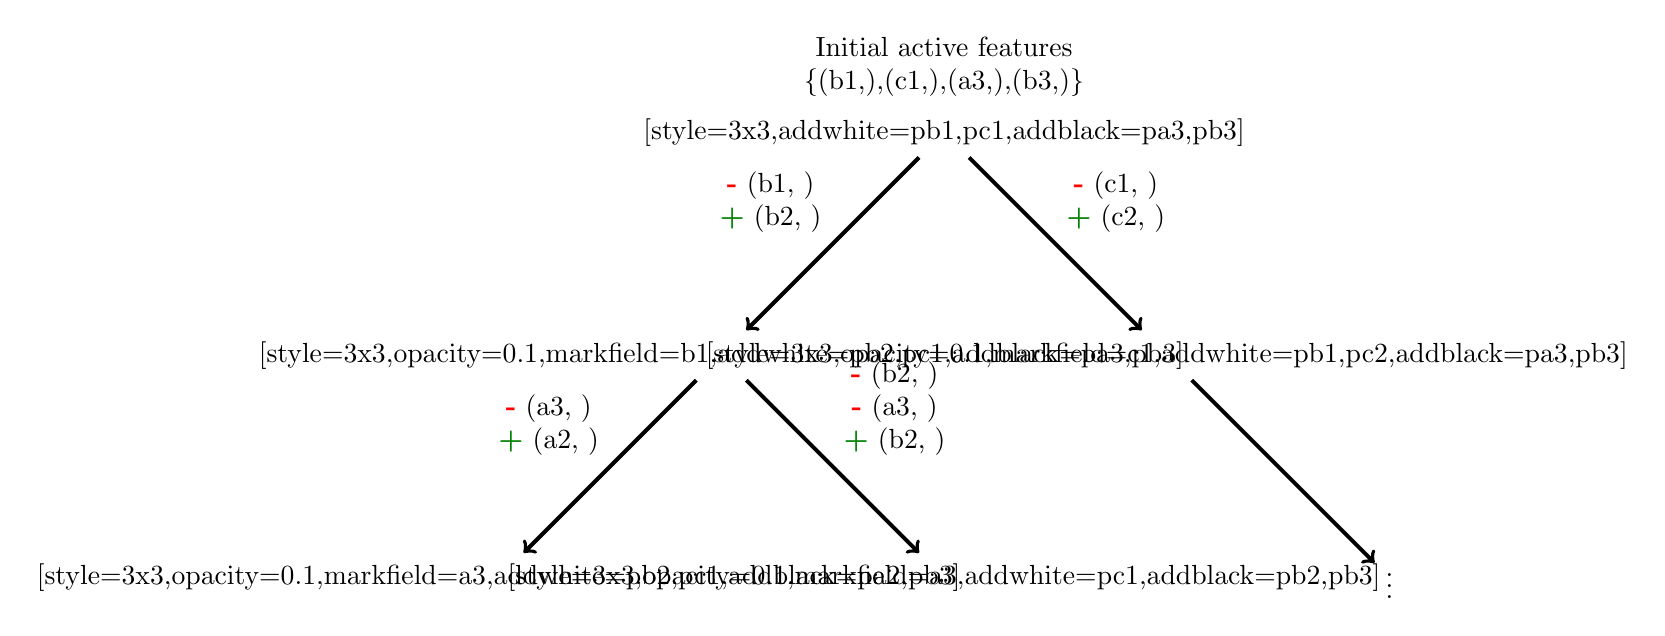
\begin{tikzpicture}[
    node distance=4cm,
    line width=0.5mm,
    auto
]

    \node[label={[align=center]Initial active features \\ \{(b1,\white),(c1,\white),(a3,\black),(b3,\black)\}}] (A) {\chessboard[style=3x3,addwhite={pb1,pc1},addblack={pa3,pb3}]};

    % childs of A
    \node (B) [below left of=A] {\chessboard[style=3x3,opacity=0.1,markfield={b1},addwhite={pb2,pc1},addblack={pa3,pb3}]};
    \node (C) [below right of=A] {\chessboard[style=3x3,opacity=0.1,markfield={c1},addwhite={pb1,pc2},addblack={pa3,pb3}]};

    % childs of B
    \node (D) [below left of=B] {\chessboard[style=3x3,opacity=0.1,markfield={a3},addwhite={pb2,pc1},addblack={pa2,pb3}]};
    \node (E) [below right of=B] {\chessboard[style=3x3,opacity=0.1,markfield={a3},addwhite={pc1},addblack={pb2,pb3}]};

    % childs of C
    \node (F) [below right of=C] {\vdots};

    % arrows of A
    \path[<-] (B) edge node[align=center] {\textbf{{\color{Red}-}} (b1, \white) \\ \textbf{{\color{Green}+}} (b2, \white)} (A);
    \path[->] (A) edge node[align=center] {\textbf{{\color{Red}-}} (c1, \white) \\ \textbf{{\color{Green}+}} (c2, \white)} (C);
    
    % arrows of B
    \path[<-] (D) edge node[align=center] {\textbf{{\color{Red}-}} (a3, \black) \\ \textbf{{\color{Green}+}} (a2, \black)} (B);
    \path[->] (B) edge node[align=center] {\textbf{{\color{Red}-}} (b2, \white) \\ \textbf{{\color{Red}-}} (a3, \black) \\ \textbf{{\color{Green}+}} (b2, \black)} (E);

    % arrows of C
    \path[<-] (F) edge node[align=center] {} (C);

\end{tikzpicture}
\caption{Partial tree of feature updates (\textcolor{Red}{removals} and \textcolor{Green}{additions}) for $\fs{SQUARE}_P \times \fs{COLOR}_P$ in a simplified 3x3 pawn-only board.}
\label{fig:updates_tree}
\end{figure}

goes very well with incremental updates

pesada al principio y liviana al final, acumular filas de la primera capa en domove, undomove

\subsection{Stockfish quantization scheme}



\textbf{Rango de activación}: en el modelo original usamos ClippedReLU, asi que queremos que el rango vaya de 0..1 a 0..127.


Siendo $\bm{x}$, $\bm{w}$ y $\bm{b}$ los parámetros de una capa lineal sin cuantizar e $\bm{y}$ la salida de la misma, se tiene que:

\begin{equation}
\begin{aligned}
\bm{y} &= \bm{x} \bm{w} + \bm{b} \\
s_a s_w \bm{y} &= (s_a \bm{x}) (s_w \bm{w}) + s_a s_w \bm{b} \\
\end{aligned}
\end{equation}



\vspace{1cm}
$s_o ((s_a \bm{x}) (s_w \bm{w}) + s_a s_w \bm{b}) = s_a s_w s_o \bm{y}$



\subsection{Network sparsity}

o combinar con 3.2?
poner graficos con la sparsity de cada feature set, decir que es muy esparso todo y que se podría mejorar aún más

\section{Engine implementation}

:)

stockfish too complicated :)
\section{Training}

Given a feature set, the network architecture is completely defined, along with how to encode a position into its inputs. This section will describes two proposed methods to train the networks, each with its own loss function and training dataset.

\subsection{Source dataset}

Data is needed to train the network. The proposal for the thesis was to use the Lichess database \cite{lichessdb}, which provides a CC0 database with all the games ever played on the site, then score the positions using Stockfish. After some initial experiments, the networks were not performing as expected. Upon further reaserch I found out that I was working with datasets too small for this task (order of hundreds of millions). I needed a larger dataset (order of \textbf{dozens of billions}), but it was impractical for me to generate it. Fortunately, I can use the same dataset that Stockfish uses to train its networks \cite{sf_nnue_dataset}, which should work well. Specifically, I went with the dataset used to train the first stage of the main network for Stockfish 16.1, which is 135GB of compressed \texttt{binpack} files. It was built by running Stockfish at 5000 nodes per move on multiple opening books. Later stages use datasets generated by Leela Chess Zero (LC0), which is more expensive to compute but has a higher quality evaluations.

The \texttt{binpack} format is a very efficient format to store samples yet very complex to decode. Fortunately, Stockfish provides a tool to export this data into a text format. I had to modify it to export it in the format I wanted. I changed the \texttt{emitPlainEntry} function in \texttt{nnue\_data\_binpack\_format.h} to the code in Appendix \ref{appendix:emitPlainEntry}. The resulting file was 2.59TB in size and contained \textbf{48.4 billion samples}. There is one sample per line with the format:

\begin{center}
\begin{tabular}{|cp{0.0005cm}cp{0.0005cm}c|}
\hline
\textbf{FEN\footnotemark} & , & \textbf{Score} & , & \textbf{Best move} \\
\hline
\end{tabular}
\end{center}

\footnotetext{Standard notation to describe positions of a chess game. It is a sequence of ASCII characters.}

The file was too big to be practical and it would wear off my SSD, so I made a tool to compact the data into a similar format. The new format expoits the fact that samples in a row belong to the same game. This means that contiguous FENs are a move from a previous one, so it stores the move instead of the FEN:

\begin{center}
\begin{tabular}{|cp{0.0005cm}cp{0.0005cm}c|}
\hline
\textbf{FEN} & , & \textbf{Score} & , & \textbf{Best move} \\
\hline
\end{tabular}
(
\begin{tabular}{|p{0.0005cm}cp{0.0005cm}cp{0.0005cm}c|}
\hline
, & \textbf{Actual move} & , & \textbf{Score} & , & \textbf{Best move} \\
\hline
\end{tabular}
) *\footnote{Repeated zero or more times.}
\end{center}

As you can see, the new format is compatible with the last one, so only one reader was implemented. After compacting the data, the file went down to a manageable 522GB. Also, reading a single FEN and later apply moves to it is much faster than parsing a FEN every time. \\

There are many positions in the dataset that are known to not be good for training. Remember that the engine is doing quiescent search, so it does a smaller search looking for quiet positions to evaluate. This means that positions where the best move is a capture, or there is a check are filtered out when building the training batch. \\

Each training method will generate a new derived dataset based on this samples.

% Lichess is a free online site to play chess, and thankfully it provides a CC0 database \cite{lichessdb} with all the games ever played on the site. It consists of serveral compressed PGN files\footnote{Portable Game Notation: a textual format to store chess games (moves and metadata)} splitted by month since 2013, that add up to $1.71$TB compressed. The whole database contains over 5.5 billion games, that equates to around 200 billion positions. In practice, that many positions are too much to handle so I'll use only a fraction of them and take only one sample per game to increase the diversity of positions.

% The Lichess database also provides a database of puzzles
% hablar de esto en otro lado (results? eval?)

% A single game can have lots of positions, most of which are shared with millions of other games, mostly during the early game. This is a problem of its own: trying to sample positions from a game with a suitable distribution. In this work, I have chosen to only consider positions 20 half-moves into the game.

\subsection{Method 1: Score target}

The main method to train the network will use the scores provided in the dataset as target. I expect the networks to learn to predict the evaluation of a position as Stockfish would do.

\setcounter{secnumdepth}{4}
\subsubsection{Score-space to WDL-space}

Scores are values ranging from -10000 to 10000. [hablar de que score vs performance ajusta a una sigmoid]
[hablar de que se necesita una escala]

% I guess it is to steer the old network to the new one while making 
% The evaluations from Stockfish are in centipawns, which is not the exact number the network has to use as target.
% decir que no usamos el outcome de la partida para el score

\subsubsection{Loss function}

The loss function is a mean square errror with a power of 2.6 (the value used by the Stockfish's official trainer) given by

% q = (output / out_scaling).sigmoid()
% p = (target / in_scaling).sigmoid()
% loss = torch.pow(torch.abs(p - q), 2.6).mean()

\[
L(y,f(x,\bm{W}))= \left| \sigma\left(\frac{y}{\text{scale}_{\text{in}}}\right) - \sigma\left(\frac{f(x,\bm{W})}{\text{scale}_{\text{out}}}\right) \right| ^{2.6}
\]


where\dots

\begin{enumerate}
\itemsep0em
\item $y$ is the target score.
\item $f$ is the model.
\item $\bm{W}$ are the parameters of the model.
\item $x$ is the input (encoded feature set).
\item $\sigma$ is the sigmoid function.
\item $\text{scale}_{\text{in}}$, $\text{scale}_{\text{out}}$ are the scaling factors of the scores.
\end{enumerate}

\subsection{Method 2: PQR triplets}

This is an additional technique I wanted to try, described in \cite{dlchess:2014}. The method is based in the assumption that moves in the dataset are optimal. In the blog they used human moves from the Lichess database \cite{lichessdb}, so they rely in that humans make optimal or near-optimal moves most of the time, even if they are amateurs. In my case I will use Stockfish moves, which are extremely good. This method does not use the scores provided, it will have to learn them from scratch. Of course this is way harder to train but I'm curious to see how far the following idea can go.

Remember that we are trying to obtain a function $f$ (the model) to give an evaluation of a position. The idea is based on the following two principles:

\begin{enumerate}
\item For two position in succession $p \rightarrow q$ observed in the game, we will have $f(p)=-f(q)$. This comes from the fact that the game is zero-sum.
\item Going from $p$, not to $q$, but to a \textit{random} position $p \rightarrow r$, we must have $f(r) > f(q)$ because the random move is better for the next player and worse for the player that made the move.
\end{enumerate}

If this reasonable assumptions hold, a loss function that expresses the equality and inequality can be built.

% Consider an optimal $f$, that outputs $-1,0,1$ depending on who wins.
% With infinite compute, $f$ would be the result of running minimax to the end of the game, since minimax always finds optimal moves.

\subsubsection{Loss function}

The loss function is the log likelihood of the inequalities: $f(r) > f(q)$, $f(p) > - f(q)$ and $f(p) < -f(q)$. The last two are a way to express the equality $f(p)=-f(q)$. The loss function is given by

% p = output[:,0] / out_scaling
% q = output[:,1] / out_scaling
% r = output[:,2] / out_scaling
% a = -torch.log(torch.sigmoid(q - r)).mean()
% b = -torch.log(torch.sigmoid((p + q))).mean()
% c = -torch.log(torch.sigmoid((-q - p))).mean()
% loss = a + b + c

\begin{align*}
L(x_p, x_q, x_r, \bm{W})=
& -\log\left(\sigma(q - r)\right) \\
& -\log\left(\sigma(p + q)\right) \\
& -\log\left(\sigma(-(p + q))\right)
\end{align*}

where\dots

\begin{enumerate}
\itemsep0em
\item $
p = \frac{f(x_p, \bm{W})}{\text{scale}_{\text{out}}},\text{ }
q = \frac{f(x_q, \bm{W})}{\text{scale}_{\text{out}}},\text{ }
r = \frac{f(x_r, \bm{W})}{\text{scale}_{\text{out}}}
$
\item $f$ is the model.
\item $\bm{W}$ are the parameters of the model.
\item $x_i$ is the input (encoded feature set) for the $i \in \{p,q,r\}$ position.
\item $\sigma$ is the sigmoid function.
\item $\text{scale}_{\text{out}}$ are the scaling factors of the scores.
\end{enumerate}

It is important to note that quantization is happening in this method too, so the output of the model must be scaled appropriately.

[siento que falta explicar algo en esta seccion]

\subsection{Setup}

[a esta seccion se le pueden agregar mil cosas]

% [multithreaded, perf]
% decir que en "All" tengo 450 it/s (7.3M pos/sec)


The project is written in two languages: Rust and Python. The Rust part is used to process dataset files, generate statistics and provide final training batches for Python to consume. The Python part defines the Pytorch model, runs the training loop, quantizes the model and runs the evaluations.


The training process is started by running a Python script (\texttt{scrips/train.py}) and it requires to define the model architecture (number of neurons on each layer), general training parameters (learning rate, batch size, epochs, checkpoints, etc) and the feature set to use, which in turn determines the size of the batches. For example, if PQR is used, the size of a sample is 3 times the size of the feature set times two (because it is siamese), and if it is eval (short for score \textbf{eval}uations), it is the size of the feature set times two plus 1 for the target score.

To orchestrate training runs, the platform Weights and Biases (WandB) is used. It provides automatic sweeping of hyperparameter, logging of metrics and visualizations. Results are exported from the platform in CSV and then processed by Python scripts. \\

% multithreading
AAAA M \\

The training data has to be converted to an actual tensor of floats to be consumed by Pytorch. This is done by a Rust subprocess running the subcommand \texttt{samples-service} that read the training data files and generates training batches for the specified feature set in a shared memory buffer. The Python script copies the data from the buffer at the start of each iteration, allowing Rust to generate the next batch (in the CPU) while Pytorch is training the current batch (in the GPU). To coordinate the memory access between the two processes, a single byte is sent using standard I/O.

Given that the input vector is multiple-hot encoded, the data written by the Rust process are not float values. Instead, they are 64-bit integers acting as a bitset. Before passing the vector to the model, it is expanded into floats. This means 64 floats can be packed into a single 64-bit integer, meaning a \textbf{96.875\%} reduction in memory usage (from 256 to 8 bytes). The speedup obtained by this optimization was substantial. The compression can be further improved using sparse tensors, but it is not implemented in this work. \\

[evaluation?]


\section{Results}


\subsection{Active neurons}

medir si hay feature sets que no usen neuronas, que esto disparo el uso de HalfTopK

average number of features enabled by feature set (cantidad y porcentaje)

\section{Final words}
\subsection{Conclusions}
\subsection{Future work}


% prunning feature sets? quizas no ayuda, solo para training, no se. ver bien

% lo ideal de un feature set son patrones que NO se den en simultáneo? asi podes aprender mas usando menos neuronas

future work: hacer que no sea uniforme el sampling de las posiciones para armar los datasets

future work: triplet loss?

deduplication de posiciones (al computar el score de Stockfish)


\newpage
\printbibliography

\end{document}


% orden de escritura:
% encodings
% training
% results
% el resto...

% https://ctan.dcc.uchile.cl/info/symbols/comprehensive/symbols-a4.pdf